%matplotlib inline: esto es para que las graficas aparescan a dentro.

\documentclass{article}
%Reporte de computacional
%matplotlib inline: esto es para que las graficas aparescan a dentro.
\usepackage{hyperref}
\usepackage{amsmath}
\usepackage{amsthm}
\usepackage{amssymb}
\usepackage{graphicx}
\usepackage{ifxetex}
\ifxetex
\usepackage{fontspec}
\else
\usepackage[T1]{fontenc}
\usepackage[utf8]{inputec}
\usepackage{lmodern}
\fi



\begin{document}
\title{ }
\author{Ramses Pacheco Ortiz}
\date{26 de Abril Del 2018}
\maketitle  


\section{Introducción}

En esta parte del curso empezaremos un tema nuevo,con un nuevo plataforma de trabajo llamdo \textbf{"Maxima"}.Este reporte consistira en aprender a utilizar esta plataformapor medio de un tutorial.

\vspace{.1cm}

Comenzaremos describiendo que es Maxima y sus caracteristicas:

Maxima es un sistema de álgebra computacional, o CAS para abreviar, es una pieza de software matemático. Permite a un usuario (que es nosotros) escribir
Preguntas sobre Álgebra, Cálculo y Estadísticas: utilizando comandos que son razonablemente similares al lenguaje humano,e intenta responderlos usando el poder computacional de la computadora.

Una de las CAS más antiguas que existe es una llamada Macsyma. Comenzó su vida de software en 1968 por investigaciones en el MIT,Macsyma fue originalmente diseñado para ser ejecutado en una línea de comando - solo texto, de echo wxMaxima es la cara bonita de la vieja escuela Maxima CAS.

\vspace{0.1cm}

Algunos comandos cortos que puedan mejor el funcionamiento de la platafroma son los sigueintes:

\begin{itemize}
\item crtl+1
 
 
 lo que hace este comando es crearte una nueva caja de texto u otra perilla

\item crtl+2 

Lo que hace este comando es agregar un titulo en tu texto

\item  ctrl+3


Lo que hace este comando es agragar una nueva sección para agregar un titulo


\item ctrl+4


Lo que hace este comando es agregar un subtitulo




\end{itemize}


\section{Aritmetica}

Cuando tu introduces algo fuera de la celda de texto maxima piensaque introduciras un comando,para evaluar el comando utilizado daremos (shift+enter) y si solomante queremos que sean una lista de instrucciones daremos solamente enter para agregar mas comandos ,a si como se observa en la figura siguiente:

\begin{center}
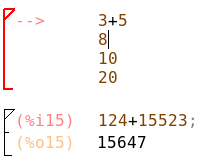
\includegraphics[height=5cm]{fto1.png}
\end{center}

como observaras en la foto el ($\%o15$) es el resultado del comando introducido,y puedes utilizarlo en mas comandos introduciendo el siguinte comando:

\begin{center}
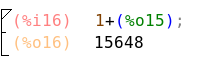
\includegraphics[height=2cm]{fto2.png}
\end{center}

Algunas veces no quieres que te muestre el resultado y para realizar esto simplemente tienes que poner el signo de pesos al final y si por algun motivo deseas que te muestre el resultado solamente introduce el(\%),en la siguiente foto ejemplifica lo anterior:


\begin{center}
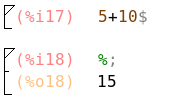
\includegraphics[height=3cm]{fto3.png}
\end{center}


Tambien muchas vesces escribes un comando y se imprime de una manera no tan leible o "bonita" y su solucion es poner una comilla(') al inicio del comando, acontinuacion se muestra un ejmplo de esto:


\begin{center}
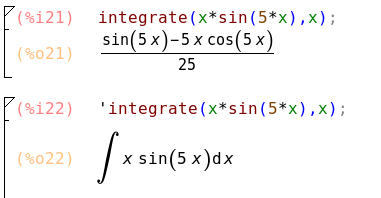
\includegraphics[height=3cm]{fto4.png}
\end{center}

\subsection{Signos de Operaciones}

Algunos de los signos de operaciones de la aritemica son los sigueintes:

\begin{itemize}
\item Adición

+

\item substracción

-

\item Multiplicacion

*

\item Division

/

\item exponente

%\^

\item Raiz

 sqrt()
 
 
\item Raiz a la n

%$\^(1/N)$ 



\end{itemize}


Otro apartado importante es al momento de realizar una fracción, puedes modificar los numeros decimales que deseas, de la siguiente manera:

\begin{center}
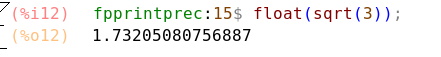
\includegraphics[height=1cm]{fto5.png}
\end{center}


Tambien puedes utilizar las constantes de pi o de euler(e)
como las siguiente imagen:


\begin{center}
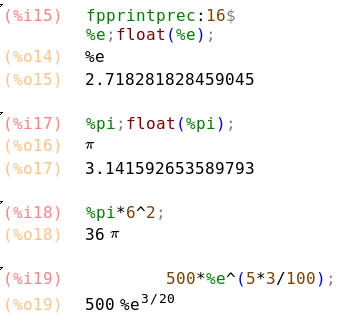
\includegraphics[height=6cm]{fto7.png}
\end{center}

\subsection{simplificando y expandiendo expreciones racionales}


En esta seccion muchas veces nosotros queremos introducir una ecuacion por ejemplo $(x+2)^2$ pero la queremos desarrollada entonces insertando el comando \textbf{"expanding"} podemos llevar acabo la accion ,en la siguiente imagen semuestra dicha accion:


\begin{center}
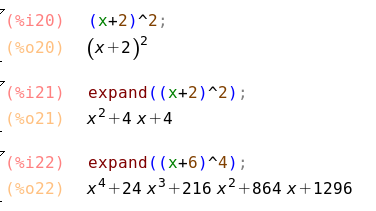
\includegraphics[height=4cm]{fto8.png}
\end{center}

En el caso anterior de la imagen, podemos enconttrar dicho factor o reducir cierto polinomo utilizando el comando \textbf{"factor"} como se muestra en la figura:

\begin{center}
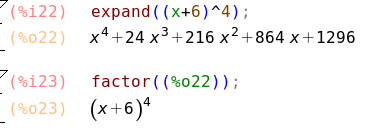
\includegraphics[height=3cm]{fto9.png}
\end{center}


otro comando importante relacionado a esto es realizar un resta de polinomios con el comando "ratsimp" lo podemos realizar como la siguiente imagen al igual que lo podemos reducir el racional resultante:

\begin{center}
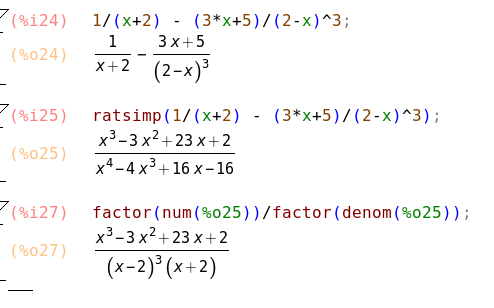
\includegraphics[height=5cm]{fto11.png}
\end{center}


\section{Funciones,Variables y ecuaciones}

\subsection{Variables}
En esta sección comenzaremos por ver las variables,la siguiente imagen muestras como introducir una variable:


\begin{center}
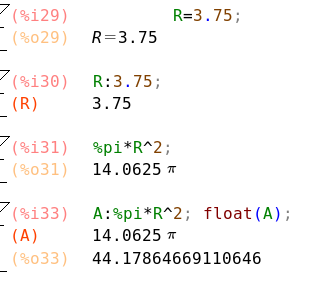
\includegraphics[height=4cm]{fto12.png}
\end{center}

tambien podemos como cancelar ciertas variables que hemos definido utilizando el comando \textbf{"kill"}, la siguiente imagen muestras un ejemplo:

\begin{center}
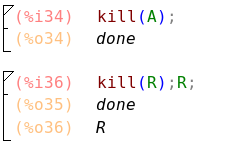
\includegraphics[height=3cm]{fto13.png}
\end{center}

\subsection{Funciones}
Para crear una funcion en maxima introduciremos el comando siguiente por ejemplo,f(x):=$(x^2+5)$ los dos puntos significa que se guarfa como funcion, un ejemṕlo de esto seria en la siguiente imagen:


\begin{center}
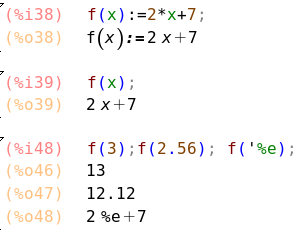
\includegraphics[height=5cm]{fto14.png}
\end{center}


Tambien podemos realizar funciones compuestas, acontinuación se mostrara por medio de la siguiente imagen:


\begin{center}
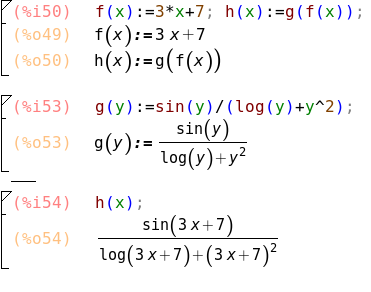
\includegraphics[height=5cm]{fto15.png}
\end{center}

\subsection{Ecuaciones}

Para realizar una ecuación o escribir una ecuacion se hace de una manera similar a las funciones, como se muestra en la siguiente imagen:

\begin{center}
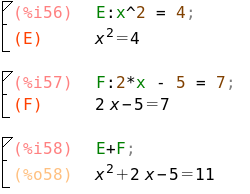
\includegraphics[height=5cm]{fto16.png}
\end{center}

\subsubsection{Solucion de ecuaciones}

Para la solucion de ecuaciones utilizaremos el comando \textbf{"solve" }y luego pondremos una coma y la variable que queremos conocer la solucion de dicha ecuacion,la siguiente figura ejemplifica lo anterior:


\begin{center}
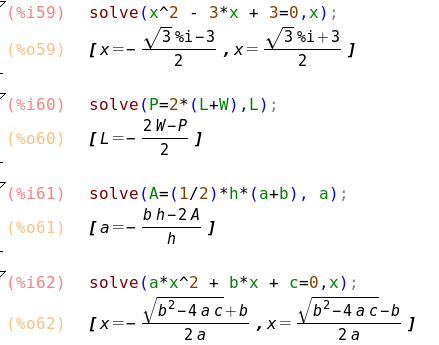
\includegraphics[height=5cm]{fto18.png}
\end{center}


\section{Graficando en Maxima}

Para graficar una funcion de manera sencilla, utrilizaremos el siguiente comando o formato\textbf{"wxplot2d(f(x),[x,xmin,xmax]) " 
}, mas adelante le agregaremos mas funciones en un mismo plano y con leyenda en los ejes,etc.

\begin{center}
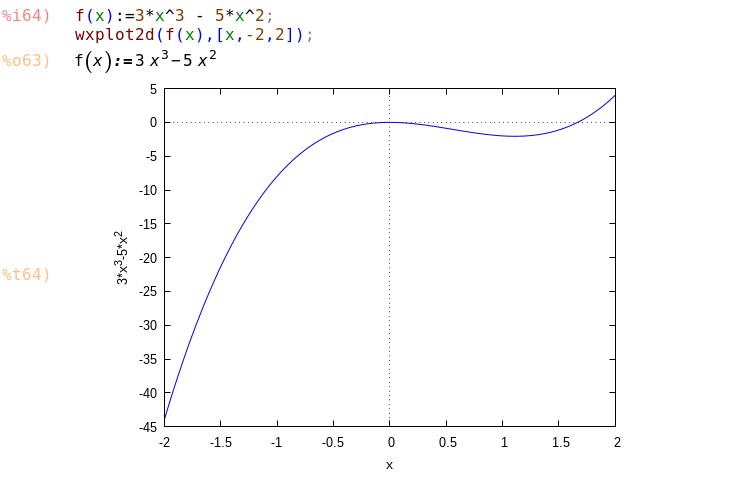
\includegraphics[height=9cm]{fto19.png}
\end{center}

Para mejorar la grafica ahora le agregaremos leyenda a los jes y le modificaremos los intervalos,le pondremos titulos,de la siguiente manera como lo muestra la imagen:

\begin{center}
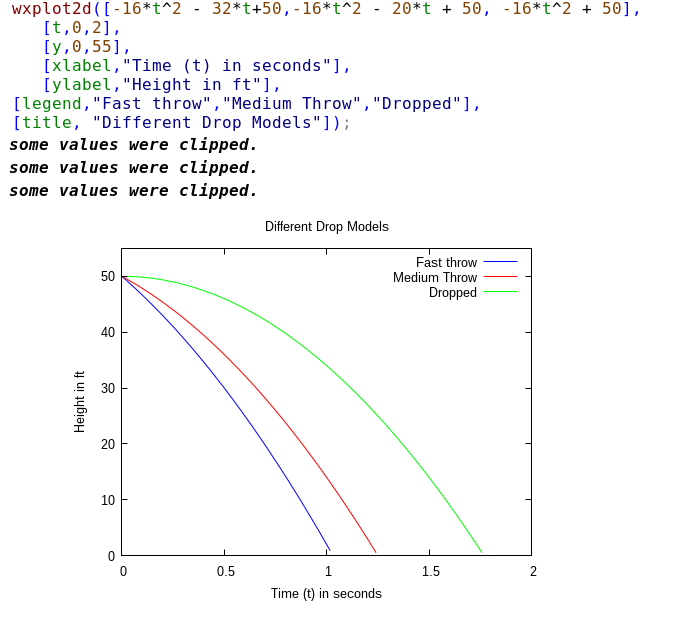
\includegraphics[height=10cm]{fto20.png}
\end{center}


Por ultimo al seleccionar la grafica podemos guardarla o copiarla.


\section{Derivadas}
\subsection{introducción}

El comando para la derivada es diff() y tiene la siguiente sintaxis diff(expression, variable, [order-of-derivative (only if greater than 1)]), un ejemplo de esto es el siguiente, el ultimo numero se refiere a los grados de derivadas, entoces serie la derivada de tal función con respecto a tal variable y cuantas veces la deriva,un ejemplo de esto es la siguiente imagen:

\begin{center}
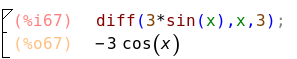
\includegraphics[height=2cm]{fto22.png}
\end{center}


\subsection{Utlizando la salidad en un nueva funcion}

Digamos que queremos diferenciar una función y luego encontrar dónde su derivada es cero, y también queremos calcular algunos valores de la derivada. Necesitamos poder "atrapar" la derivada de esa función como una nueva función. Así es como lo hacemos:


\begin{center}
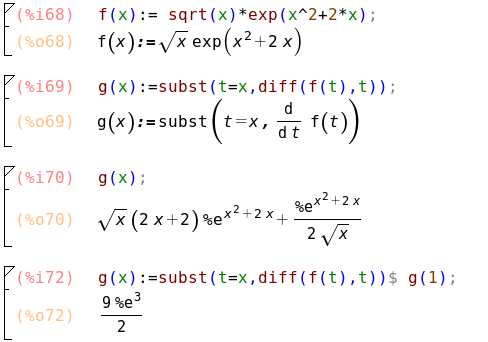
\includegraphics[height=6cm]{fto23.png}
\end{center}

\subsection{Graficando Derivadas}


Ahora que podemos atrapar derivados en sus propias funciones, podemos hacer todas las cosas habituales que nos gustaría con ellos. Por ejemplo, podríamos graficarlos junto con sus funciones, de la siguiente manera:

\begin{center}
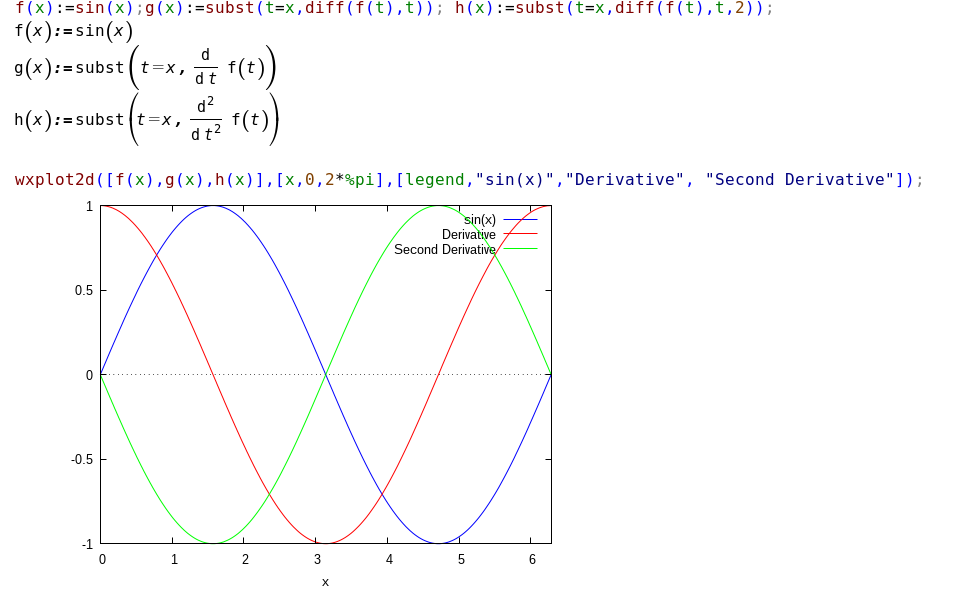
\includegraphics[height=9cm]{fto24.png}
\end{center}


\subsection{Obteniendo Valores Numericos}

Para obtener el valor numerico de una evaluacion de alguna derivada introduciremos lo siguiente:


\begin{center}
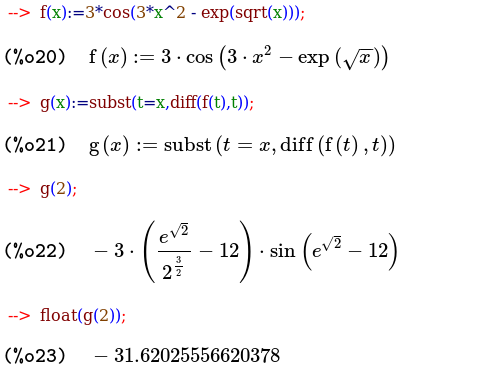
\includegraphics[height=6cm]{fto25.png}
\end{center}

el float es para los numeros en decimal.


\section{Integración}

\subsection{Integracion Basica}

\subsubsection{Integrales Indefinidas}

El comando para preformar una integral indefinida y definida es el mismo en Maxima. Para preformar una integral indefinida usamos el comando integrate (f (x), x). Tenga en cuenta que la primera entrada es la función que deseamos integrar, mientras que la segunda es la variable de integración.


\begin{center}
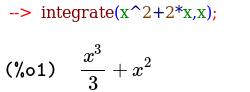
\includegraphics[height=2cm]{fto26.png}
\end{center}

para expresar la integral con su simbolo y su reasultado realizaremo lo siguiente:


\begin{center}
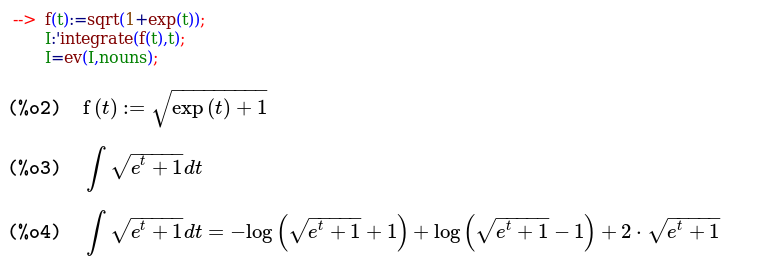
\includegraphics[height=5cm]{fto27.png}
\end{center}


\subsubsection{La Antiderivada}

Para encontrar una antiderivada es muy facíl integrar una funcion asi como lo hicimos en la seccion pasada pero ahora nos encontramos con un problema, cuando queramos evaluar no podremos poniedo solamente f(3)=..., esto parece como error, entonces lo que tenemos que hacer es lo siguiente:

\begin{center}
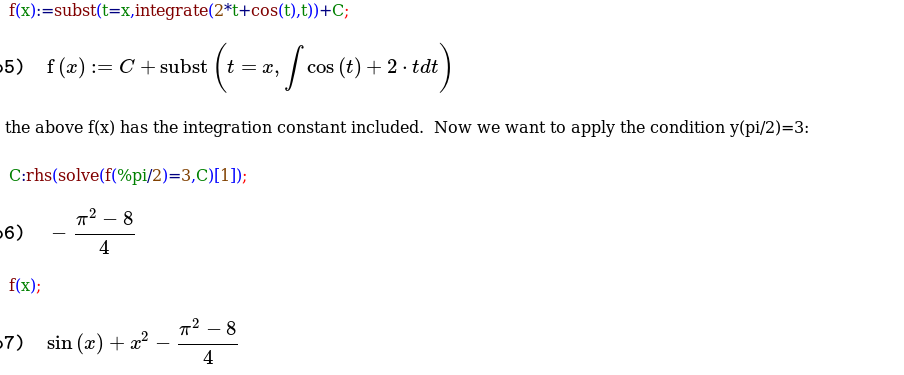
\includegraphics[height=6cm]{fto28.png}
\end{center}


\subsection{Integrales Definidas}

Para las integrales definidas la sintaxis es la siguiente:
integrate(funcion,variable a integrar,limite inferior,limite superior).A continuación veremos unos ejemplos:


\begin{center}
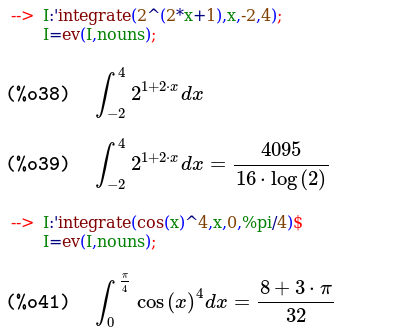
\includegraphics[height=6cm]{fto29.png}
\end{center}


\subsection{Integracion Numerica}


Digamos que no estamos tan interesados en el valor simbólico de una integral definida, sino en el valor numérico. Maxima tiene varios métodos de integración numérica. El más útil y eficiente es quad\_qags ().

A continuacion se muestra un ejemplo para ver como funciona


\begin{center}
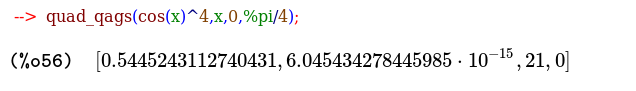
\includegraphics[height=2cm]{fto30.png}
\end{center}


quad\_qags es un método numérico que utiliza funciones cuadraticas para aproximar de forma adaptativa la función a fin de proporcionar una aproximación de gran precisión a la integral. Tenga en cuenta que el resultado viene en una lista con 4 elementos. El primero es el valor aproximado real de la integral. El segundo es el estimado de error máximo. El tercero es información sobre el número de funciones cuadráticas utilizadas para aproximar la curva, y el último elemento proporciona un código de tipo ERROR.

Pero si solamente queremos  los primeros 2 elementos, acontinuación se muestra como hacerlo:


\begin{center}
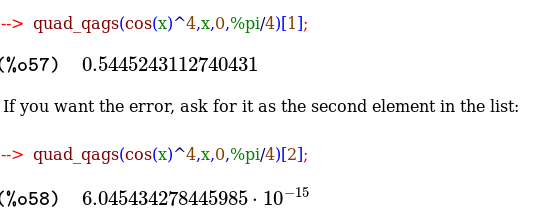
\includegraphics[height=5cm]{fto31.png}
\end{center}


En la imagen anterior el ultimo numero encerrado en corchetes es el elemento que te mostrara.


\section{Conclusion}


Nunca habia utilizado maxima y con su uso en esta practica creo que este tutorial nos servira mucho al mometo de integrar o derivar o simplemente graficar ya que Maxima trabaja muy bien en estas areas, tambien hay otras aplicaciones que realizan lo mismo pero su estilo me paracio muy facil y la plataforma muy accesible.


\section{Apéndice}
\begin{itemize}
\item \textbf{¿Cuál fue tu primera impresión de wxmaxima?}

Me parecio muy interesante la facilidad de trabajar con la plataforma y lo facil que era llevar ciertar operaciones acabo como por ejemplo fraficar un funcion,derivar,obtener raices de un polinomio ,etc.

\vspace{0.1cm}


\item \textbf{¿Crees que esta herramienta puede ser útil en otros de tus cursos?}

Por supuesot que si ya que mas adelante tendremos que realizar algunas integrales muy largas, y con esta herramienta nos facilitaria mucho las cosas 

\vspace{0.1cm}


\item \textbf{ ¿Qué se te dificultó mas en esta actividad?}

Me paracio un poco confuso al momento de ver las derivadas ya que no entendia muy bien como funcionaba cierto codigo


\vspace{0.1cm}

\item \textbf{ ¿Se te hizo compleja esta actividad? ¿Cómo la mejorarías? }


Me parecio bien, y creo que en esta actividad depende del alumno que tanto se profundizo en aprender maxima para decir si estubo pesada o no, a mi me paracio muy interesante y me sorprendio la herramienta con lo facil en que se pueden llevar a relizar ciertas operaciones.


\end{itemize}
 

\section{Bibliografia}

http://www.scotchildress.com/wxmaxima/







\end{document}